\documentclass[conference]{IEEEtran}
\IEEEoverridecommandlockouts
% The preceding line is only needed to identify funding in the first footnote. If that is unneeded, please comment it out.
\usepackage[hidelinks]{hyperref}
\urlstyle{same}
\usepackage[spanish,es-tabla]{babel}
\usepackage{cite}
\usepackage{amsmath,amssymb,amsfonts}
\usepackage{algorithmic}
\usepackage{graphicx}
\usepackage{textcomp}
\usepackage{xcolor}
\decimalpoint
\renewcommand{\labelitemi}{$\bullet$}
\def\BibTeX{{\rm B\kern-.05em{\sc i\kern-.025em b}\kern-.08em
    T\kern-.1667em\lower.7ex\hbox{E}\kern-.125emX}}
    
    
 %-------------------------------------------------------------------------------
%                            Libreria de codigos                               %
%-------------------------------------------------------------------------------
% Paquetes necesarios
\usepackage{listings}
\usepackage{xcolor}
\usepackage{comment}

% Tipos de letra personalizadas
\def\lstbasicfont{\fontfamily{pcr}\selectfont\scriptsize}
\def\vhdlbasicfont{\fontfamily{cmtt}\selectfont\scriptsize}

% Colores personalizados
\definecolor{codegreen}{rgb}{0,0.6,0}
\definecolor{codepurple}{rgb}{0.58,0,0.82}

\definecolor{codegray}{rgb}{0.5,0.5,0.5}
\definecolor{backcolour}{rgb}{0.95,0.95,0.92}
\definecolor{codeorange}{RGB}{254, 100, 35}

% Deficion de lenguajes perzonalizados

% Definicion de lenguaje MATLAB
\lstdefinelanguage{matlabfloz}{%
  alsoletter={...},%
  morekeywords={%                             % keywords
		break,case,catch,classdef,continue,else,
		elseif,end,for,function,global,if,
		otherwise,parfor,persistent,
		return,spmd,switch,try,while,...},        % Use the matlab "iskeyword" command to get those
  comment=[l]\%,                              % comments
  morecomment=[l]...,                         % comments
  morecomment=[s]{\%\{}{\%\}},                % block comments
  morestring=[m]'                             % strings 
}[keywords,comments,strings]%

% Estilos MATLAB
\lstdefinestyle{MATLAB}{
	frame=single,
	rulecolor=\color{black},
	framexleftmargin=4mm,
	xleftmargin=2mm,
	language=matlabfloz,
  commentstyle=\color{codegreen},
  keywordstyle=\color{blue}, %magenta
  numberstyle=\tiny\color{black},
  stringstyle=\color{codepurple},
  basicstyle=\lstbasicfont\scriptsize,
  breakatwhitespace=false,         
  breaklines=true,                 
  captionpos=b,                    
  keepspaces=true,                 
  numbers=left,                    
  numbersep=5pt,                  
  showspaces=false,                
  showstringspaces=false,
  showtabs=false,                  
  tabsize=2    
}

\lstdefinestyle{PYTHON}{
	frame=single,
	rulecolor=\color{black},
	framexleftmargin=4mm,
	xleftmargin=2mm,
	language=python,
    backgroundcolor=\color{backcolour},   
    commentstyle=\color{codegreen},
    keywordstyle=\color{blue}, %magenta
    numberstyle=\tiny\color{black},
    stringstyle=\color{codeorange},
    basicstyle=\lstbasicfont\footnotesize,
    breakatwhitespace=false,         
    breaklines=true,                 
    captionpos=b,                    
    keepspaces=true,                 
    numbers=left,                    
    numbersep=5pt,                  
    showspaces=false,                
    showstringspaces=false,
    showtabs=false,                  
    tabsize=2,
    otherkeywords = {show,arange}  
}



\lstdefinestyle{BASH}{
	frame=single,
	rulecolor=\color{black},
	framexleftmargin=4mm,
	xleftmargin=2mm,
	language=bash,
    %backgroundcolor=\color{backcolour},   
    commentstyle=\color{codegreen},
    keywordstyle=\color{blue}, %magenta
    numberstyle=\tiny\color{black},
    stringstyle=\color{codeorange},
    basicstyle=\lstbasicfont\footnotesize,
    breakatwhitespace=false,         
    breaklines=true,                 
    captionpos=b,                    
    keepspaces=true,                 
    numbers=left,                    
    numbersep=5pt,                  
    showspaces=false,                
    showstringspaces=false,
    showtabs=false,                  
    tabsize=2,
    %otherkeywords = {show,arange}  
}

\renewcommand{\lstlistingname}{Código}% Listing -> Algorithm
\renewcommand{\lstlistlistingname}{Lista de códigos}% 
\begin{document}

\title{Tarea 1. Método de Newton para encontrar Máximos y Mínimos \\
%%{\footnotesize \textsuperscript{*}Note: Sub-titles are not captured in Xplore and should not be used}
}

\author{\IEEEauthorblockN{ Ciro Fabian Bermudez Marquez}
INAOE\\
Mexico, Puebla \\
\url{cirofabian.bermudez@gmail.com}
}

\maketitle

\begin{abstract}
Utilizando el método de Newton se encuentran los máximos y mínimos de la función $f(x)$, posteriormente utilizando una heurística se encontró el mínimo global.
\end{abstract}


\section{Descripción del problema}

Se tiene la función de la ecuación (\ref{ec:f}) en el rango $[0,7]$, y se desea encontrar los máximos y mínimos utilizando el método de Newton.

\begin{equation}
f(x) = (x-2)(x-5) + \sin(1.5 \pi x)
\label{ec:f}
\end{equation} 
su gráfica se muestra en la Figura \ref{fig:f}.

\begin{figure}[hbtp]
\centering
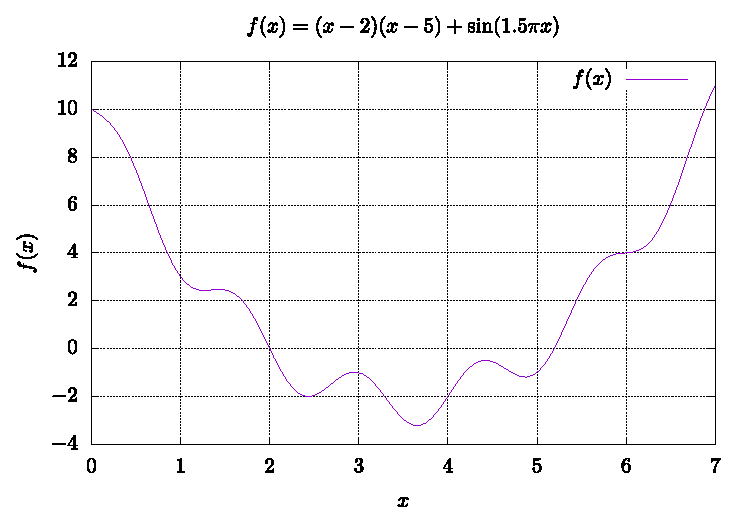
\includegraphics[width=8cm]{grafica1.eps} 
\caption{Gráfica de la función.}
\label{fig:f}
\end{figure}

\section{Método de Newton}

El método de Newton se deduce de la serie de Taylor la cual se muestra en la ecuación (\ref{ec:taylor}) y tomando los primeros dos términos obtenemos la ecuación (\ref{ec:taylor2}).

\begin{equation}
f(x) = \sum_{n=0}^{\infty} \frac{f^{(n)} (a)}{n !} (x -a)^{n}
\label{ec:taylor}
\end{equation}

\begin{equation}
f(x) = f(a) + f'(a) (x-a)
\label{ec:taylor2}
\end{equation}
si consideramos $x-a$ infinitesimal y encontrando las raíces de $f(x)$ obtenemos la ecuación (\ref{ec:alg1}) (Newton V1).

\begin{equation}
dx = - \frac{f(a)}{f'(a)}
\label{ec:alg1}
\end{equation}

Si hacemos este mismo procedimiento pero considerando $f'(x)$ para la serie de Taylor encontramos la ecuación del método de Newton para encontrar máximos y mínimos como se muestra en la ecuación (\ref{ec:alg2}) (Newton V2).

\begin{equation}
dx = - \frac{f'(a)}{f''(a)}
\label{ec:alg2}
\end{equation}
El método necesita un punto inicial $a_{0}$ para comenzar el proceso iterativo, $a_{i+1} = a_{i} + dx$ y la condición de paro son 20 iteraciones máximas o $|dx| < \epsilon$ donde $\epsilon =  1e^{-10}$.

\section{Utilización del método de Newton V2}

Para utilizar este método es necesario conocer hasta la segunda derivada de la función, las cuales se muestran en (\ref{ec:fp}) y (\ref{ec:fpp}) y en en la Figura \ref{fig:fp} se muestra la derivada de la función.

\begin{equation}
f'(x) = 2x -7 + 1.5 \pi \cos(1.5 \pi x)
\label{ec:fp}
\end{equation}

\begin{equation}
f''(x) = 2 -(1.5)^{2} \sin(1.5 \pi x)
\label{ec:fpp}
\end{equation}

\begin{figure}[hbtp]
\centering
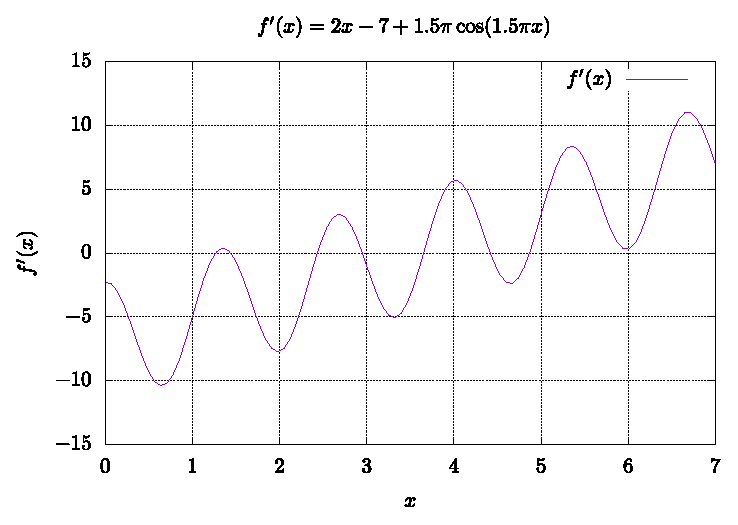
\includegraphics[width=8cm]{grafica2.eps} 
\caption{Gráfica de la derivada función.}
\label{fig:fp}
\end{figure}

Observando cuidadosamente la gráfica de la Figura \ref{fig:fp} resalta a la vista que la función es multimodal, esto significa que presenta más de un punto máximo y mínimo. La función presenta 3 mínimos locales, 3 máximos locales y un mínimo global. 

El método de Newton necesita un punto inicial para comenzar el proceso iterativo de encontrar una solución y debido a que es multimodal a menos que se elija un punto muy cercano el mínimo global el método va a converger a alguna otra solución.

\section{Resultados}

\subsection{Prueba del método de Newton V2}
Eligiendo un valor inicial $a_{0}$ cercano a los máximo y mínimos obtenemos los resultados de la Tabla \ref{tab:res1}.

	\begin{table}[h!]   
	\caption{Máximos y mínimos encontrados con el método de Newton V2.}                                                                                                                
		\centering                                       
		\begin{tabular}{ccccc}
			\hline                                             
			$a_{0}$ & $x$  & $|dx|$ & Iteraciones & Max o Min\\                     
			\hline 
			1.2 & 1.26419808  & 5.53050375e-11 & 5 & Min\\                                            
			1.4 & 1.44108574  & 1.00957580e-16  & 16 & Max\\                                            
			2.4 & 2.43305587  & 7.74529240e-13 & 4 & Min\\                                            
			2.9 & 2.95000435  & 1.39272369e-11 & 4 & Max\\                                            
			3.6 & 3.65288744  & 1.02705621e-14 & 4 &\textbf{Min Global}\\                                            
			4.4 & 4.41828865  & 1.19983916e-14 & 4 & Max\\                                            
			4.8 & 4.86849168  & 5.48555533e-15 & 5 & Min\\                                            
			\hline                                             
		\end{tabular}
		\label{tab:res1}
	\end{table}	

\subsection{Heurística para encontrar mínimo global}
La heurístaica para encontrar el mínimo global consiste en generar un punto inicial $a_{0}$ aleatorio en el rango $[0,7]$, ejecutar el método de Newton V2 y comprobar si la solución encontrada es el mínimo global utilizando el siguiente criterio:

\begin{equation}
	|x - \text{Min}_{\text{global}}| < 1e-4
\end{equation}
esto se repite 100 veces considerando que el mínimo global se encuentra en $x = 3.65288744$ y $f(x) = -3.22451801$.

De las 100 repeticiones la heuristica solo encontró el mínimo global 9 veces, esto equivale a una eficiencia del 9\%.

\section{Conclusiones}

De la aplicación de esta heurística podemos decir que el método de Newton no es muy eficiente cuando se trata de problemas multimodales, y si se desea utilizar este método para problemas de más de una variable la eficiencia podemos esperar una eficiencia aun peor.



\begin{thebibliography}{00}
\bibitem{b1}  Dr. Luis Gerardo de la Fraga. ``Apuntes de clase'' .
\end{thebibliography}


\end{document}
